\section{Lecture 9: Different Potentials}

Consider the following potential:

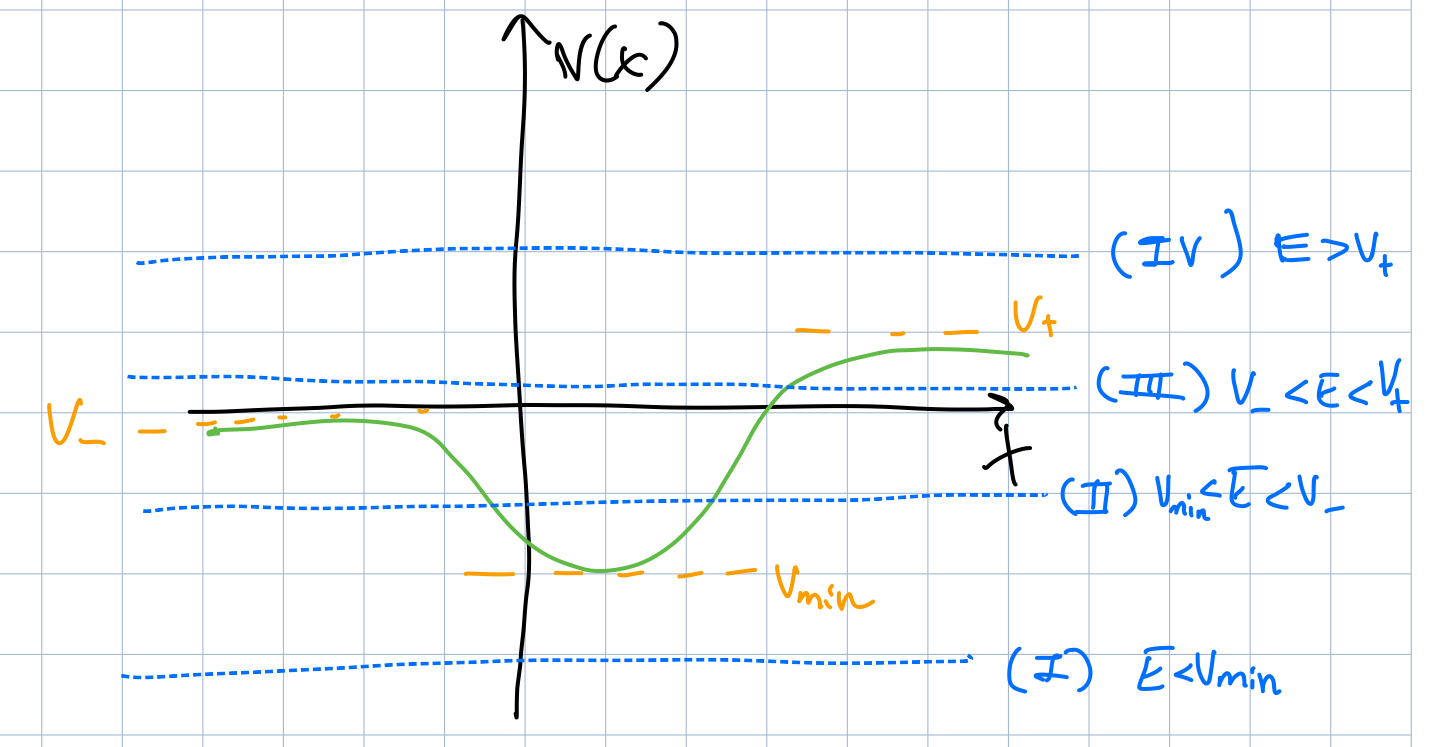
\includegraphics[width=400px]{wigglypot.jpeg}

Let us try solving the Schrodinger equation:
\[ \qty[-\frac{\hbar^2}{2m} \derivative{}{x} + V(x)] \Psi_E(x) = E \Psi_E(x) \]
We will work through the marked cases on the diagram.
\begin{enumerate}
    \item Doing a simple subtraction:
    \begin{align*}
        \derivative{^2}{x^2} \Psi(x) &= \frac{2m}{\hbar^2} (V(x) - E) \Psi(x)
    \end{align*}
    Since $V(x) - E > 0$, this means that $\derivative{^2\Psi}{x^2}$ and $\Psi$ have the same sign. But look at some candidate solutions. These
    all diverge, which would contradict normalization!
    
    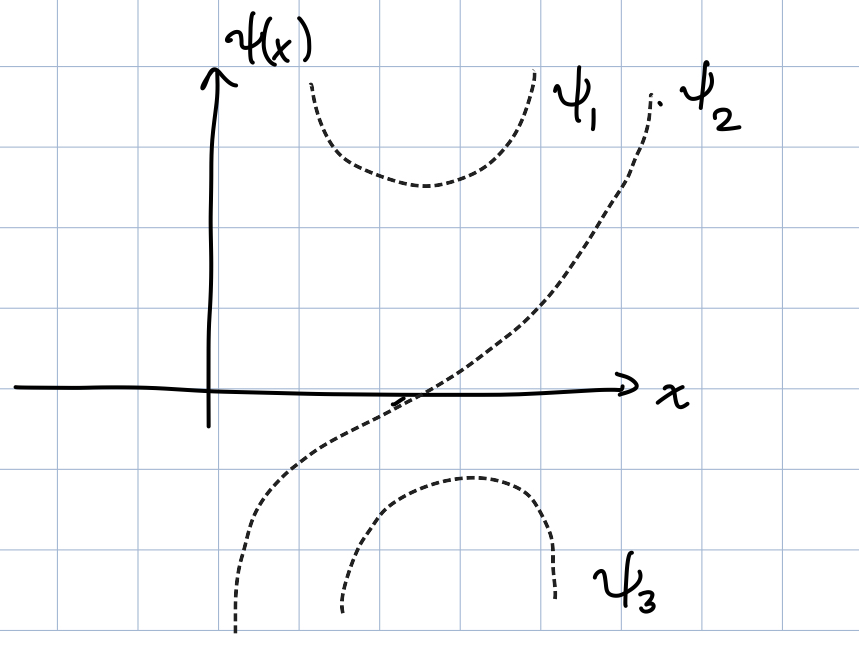
\includegraphics[width=250px]{divded.jpeg}

    No solutions for $E < V_min$, which makes sense--you can't allow states lower than the lowest energy.
    \item We detail some possibilities considering curvature:
    
    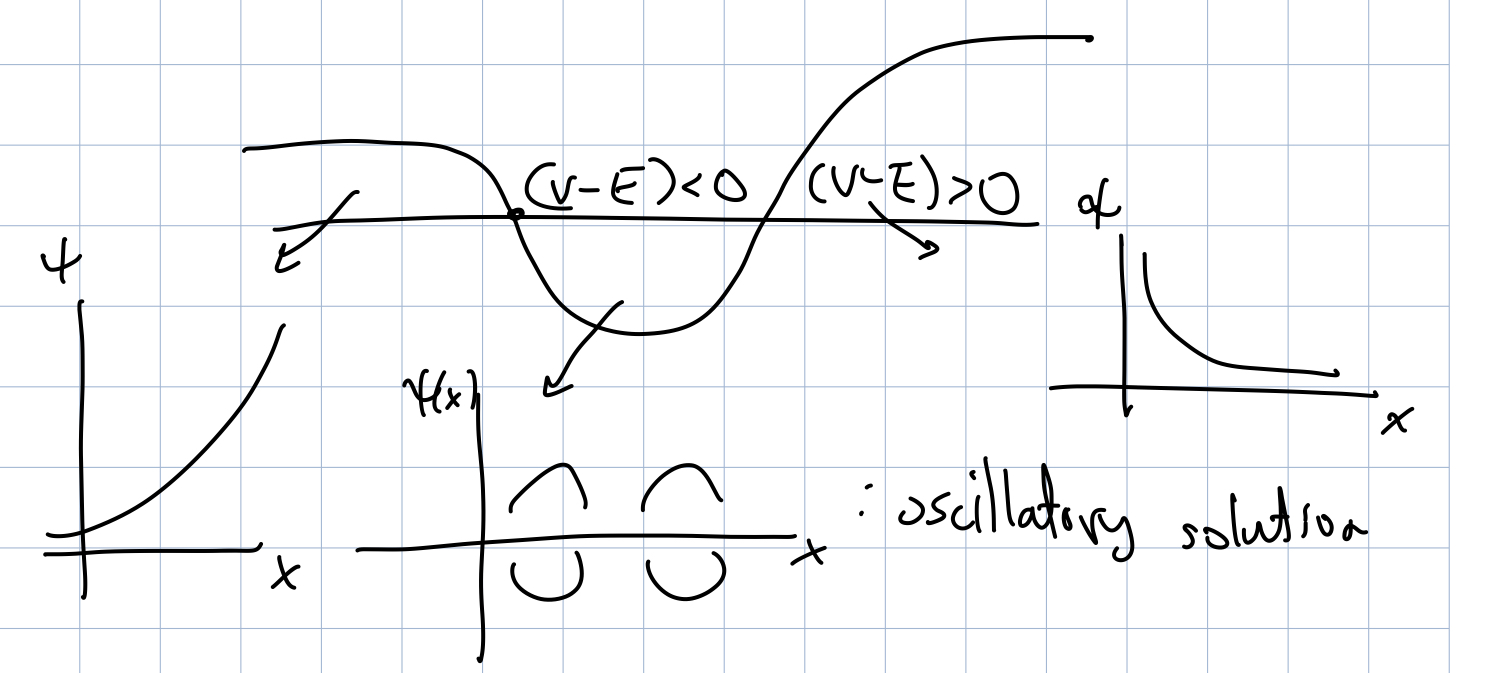
\includegraphics[width=400px]{curvoposs.jpeg}

    However, $\Psi$ and $\derivative{\Psi}{x}$ must be continuous by a probabilistic interpretation of $|\Psi|^2$. Thus a stitched solution must
    be like 

    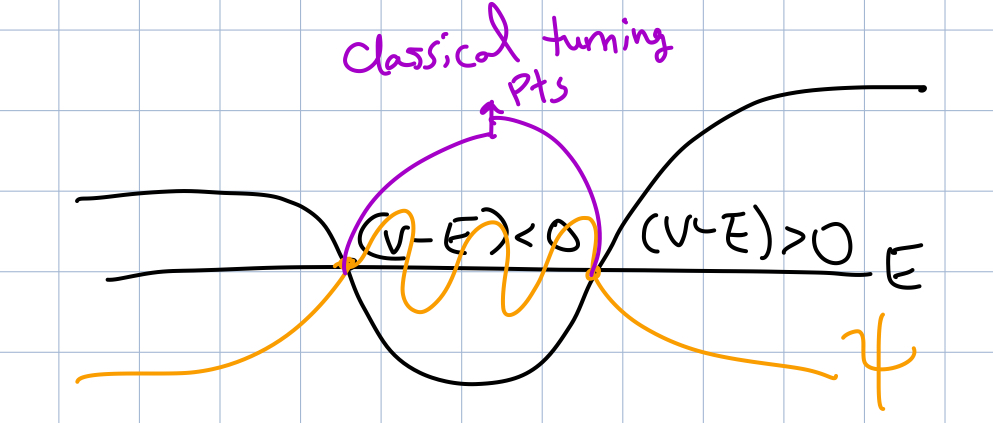
\includegraphics[width=400px]{stitching gaming.jpeg}

    Notice that at the ends there is an exponential decay! So there is a small (but vanishing) probability that
    we have the wavefunction at a lower energy than the potential!

    The oscillatory wave in the middle quantizes the allowed values of $E$ (you can only have energies that fit the boundary conditions). These are called bound states.

    \item With similar reasoning, this case looks like:
    
    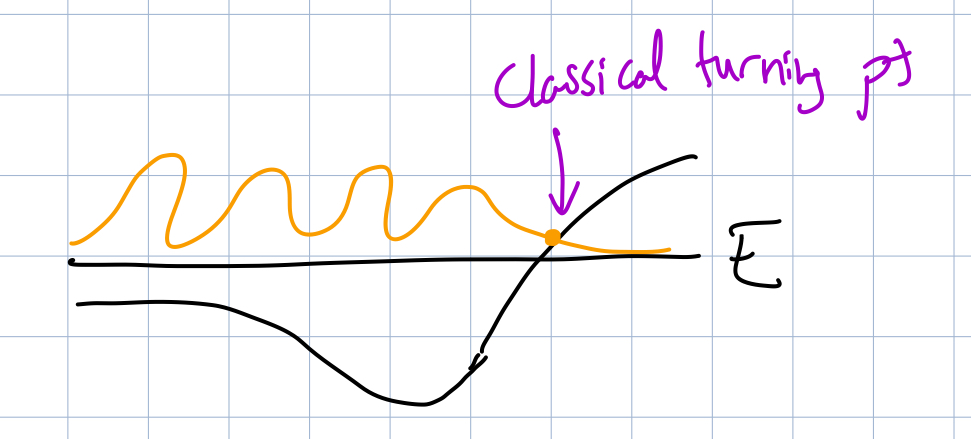
\includegraphics[width=400px]{onecurvetorulethemall.jpeg}

    However, since you only have one boundary condition for a second-order equation, there is no energy quantization! Any energy in between can be allowed.

    \item Lastly, the second-derivative is proportional to the difference, so oscillatory solutions will be faster wiggling in the lower potential reasons. They are called scattering states.
\end{enumerate}

\subsection{Free Particle, Revisited}
Let us walk through the case of a free particle ($V = 0$). We write the Time-Independent Schrodinger Equation:
\begin{align*}
    -\frac{\hbar^2}{2m} \derivative{^2 \Psi(x)}{x^2} &= E\Psi
\end{align*}
let $k = \qty(\frac{2mE}{\hbar})^{1/2}$
\begin{align*}
    \derivative{^2 \Psi(x)}{x^2} + k^2 \Psi(x) &= 0 \\
    \Psi(x) &= Ae^{ikx} + Be^{-ikx}
\end{align*}
Degeneracy in $E$ (i.e. $\Psi$ with $\pm k$ has same energy). So the eigenfunction is:
\[ \Psi_E(x, t) = (Ae^{ikx} + Be^{-ikx}) e^{-iEt/\hbar} \]

Case 1:
Suppose $B = 0$, then:
\[ \Psi(x, t) = Ae^{i(kx - \omega t)} \]
which is a traveling wave moving to the right. Probability density is $|\Psi|^2 = |A|^2$. What's the probability current?
\begin{align*}
    j &= \frac{\hbar}{2mi} \qty[\Psi^* \partialderivative{\Psi}{x} - \Psi \partialderivative{\Psi^*}{x}] \\
    &= \frac{\hbar k}{m} |A|^2 = v |A|^2
\end{align*}

Case 2:
Suppose $A = 0$, then the analysis is the same, but the traveling wave is moving to the left.

Case 3:
Suppose $A = B$, then:
\[ \Psi(x, t) = A\qty(e^{ikx} + e^{-ikx})e^{-i\omega t} = 2A \cos(kx) e^{i\omega t} \]
This is a standing wave with nodes at $x_n = \pm \frac{\frac{\pi}{2} + n \pi}{k}$ for $n \in \Z$.

How can we normalize such a wave function? We use the good old Delta Trick:
\[ \int e^{i(k - k')x} \dd{x} = 2\pi \delta(k -k') \]
which means $\Psi(x) = \frac{1}{\sqrt{2\pi}} e^{ikx}$.